\documentclass[12pt]{article}

% Packages
\usepackage[margin=1in]{geometry}
\usepackage{times}
\usepackage{graphicx}
\usepackage{booktabs}
\usepackage{amsmath}
\usepackage{amssymb}
\usepackage{float}
\usepackage{setspace}
\usepackage{natbib}
\usepackage{url}
\renewcommand{\UrlFont}{\normalsize\ttfamily}\urlstyle{same}
\usepackage{indentfirst}
\usepackage{titlesec}
\usepackage{subcaption}
\usepackage{bbm}
\usepackage{placeins}


% Set spacing and font size
\onehalfspacing
\renewcommand{\normalsize}{\fontsize{12pt}{14pt}\selectfont}
\setlength{\parindent}{0.5in}

% Format subsections (level 2 headings) - centered, italicized, not bold
\titleformat{\subsection}{\centering\normalsize\itshape}{}{0pt}{}

% Title and Author Information
\title{\normalsize The Impact of Employee Ownership Support Programs on ESOP  Participation: Evidence from Colorado's HB17-1214}
\author{\normalsize Mitchell Ballif, Patrick Beal, Will Cheney, and Soren Pack}
\date{}

\begin{document}

\maketitle

% Abstract
\begin{center}
\normalsize \textbf{ABSTRACT}
\end{center}

This paper examines the causal effect of Colorado's HB17-1214, an employee ownership support program enacted in 2017, on Employee Stock Ownership Plan (ESOP) participation. Using firm-level data from Department of Labor Form 5500 filings and a difference-in-differences design comparing Colorado to Utah, we find limited evidence of significant policy effects. Our preferred specification shows small and mostly statistically insignificant increases in ESOP participation and assets, with only total ESOP assets marginally significant at the 10\% level. While synthetic control estimates suggest larger effects, we interpret these cautiously given the fundamental identification challenges of studying a single treated state. Our findings suggest that education-based and financing-focused employee ownership policies may require longer time horizons or more direct financial incentives to generate substantial increases in ESOP adoption among small and medium-sized businesses. We discuss important methodological limitations including the inability to conduct proper state-level inference with only two states and potential confounding from Colorado-specific post-treatment trends.

\vspace{12pt}

% Roman numeral counter for sections
\renewcommand{\thesection}{\Roman{section}}
\renewcommand{\thesubsection}{\Roman{subsection}}

% I. BACKGROUND
\section*{\centering \normalsize \textbf{I. BACKGROUND}}

\subsection*{A. Employee Stock Ownership Plans}

Employee Stock Ownership Plans (ESOPs) are retirement benefit plans that enable employees to acquire ownership stakes in their employer company. Instead of giving stock directly to individual employees, ESOPs function as trusts that hold company shares on behalf of plan participants. The trust maintains individual accounts for each participant, with allocations typically vesting over three to six years. When employees leave the company, employers must repurchase the shares of the employees, making sure the assets can be liquidated for employees who leave.

ESOPs are governed by the Internal Revenue Code and the Employee Retirement Income Security Act (ERISA), which require that these plans are broad-based and nondiscriminatory (29 U.S.C. \S 1107; 26 U.S.C. \S\S 4975, 409). Specifically, ESOPs must include all full-time employees who have worked at the company for at least a year, so that companies cannot use the plans to selectively reward individual employees. These regulations mean that once a company has established an ESOP, the whole workforce is included. Employees cannot opt out of being included in the plan, nor can they select into the plan except through their choice of where to work.

Two primary types of ESOPs exist: leveraged ESOPs and non-leveraged ESOPs. Leveraged ESOPs involve taking out loans with which the trust purchases company shares. The company then makes tax-deductible contributions to pay back the loan, with both principal and interest being deductible. Significant tax benefits come from this structure. Non-leveraged ESOPs involve direct contributions of company stock or cash to buy existing shares without borrowing loans. Both structures provide tax benefits to the ESOP plan sponsor, including deductible contributions, preferential treatment of S corporation ESOP shares at the federal level, and potential deductibility of dividends.
% Prof. Wilson: I would add research question here as well or why OLS doesn't work

This paper asks: Did Colorado's HB17-1214 policy significantly increase ESOP adoption among eligible firms?  The policy introduced educational programs and loan financing infrastructure to Colorado firms starting in 2017. Most notably, it established a loan program capitalized with \$200,000 in annual state appropriations through 2022 to finance business transitions to employee ownership. Our treatment is eligibility for this \$200,000 financing option and accompanying educational resources. We compare outcomes for firms headquartered in Colorado after 2017 (treated) to firms in Utah throughout the study period and Colorado firms before 2017 (controls). 

Given the small number of ESOP adoptions annually in both states, simply comparing aggregate adoption counts would lack sufficient statistical power to detect policy effects. This motivates our use of firm-level Form 5500 data, which allows us to analyze both whether firms adopt ESOPs and the total participants and assets among adopting firms. This approach substantially increases our sample size and statistical power. A simple OLS approach would be biased because firms' ESOP adoption decisions depend on unobserved factors that vary across states and time, such as firm profitability, management preferences, and labor market conditions. To isolate the causal effect of the policy, we employ a difference-in-differences design that compares treated firms (Colorado post-2017) to control firms (Utah throughout the period, and Colorado pre-2017).

\subsection*{B. ESOP Data and Form 5500}

ERISA requires that all ESOP sponsors file Form 5500, which is the annual report of employee benefit plan information, with the U.S. Department of Labor, typically due by the end of July after the plan year. Form 5500 captures financial and operational data about the ESOP, including total assets, the number of plan participants, participant accounts, and contributions to the plan. For ESOPs specifically, Schedule E (ESOP Annual Information) must accompany the standard Form 5500 filing \citep{DOLForm5500ScheduleE}. ESOPs with 100 or more participants at the beginning of the plan year are required to attach audited financial statements to their Form 5500 filing. These public filings through the Department of Labor's EFAST2 system (\url{https://www.efast.dol.gov/}) create a comprehensive national dataset of ESOP participation and assets, making Form 5500 data a valuable empirical resource for studying the prevalence and impact of employee ownership structures at the firm level.
% Prof. Wilson: Need more about your data structure. What level? What dates? What restrictions? What info are you using and why?

\subsection*{C. Colorado HB17-1214: Legislative Support for Employee Ownership Models}

In 2017, the Colorado legislature enacted House Bill 17-1214, signed by Governor John Hickenlooper, as a policy initiative to encourage transitions of existing small businesses to employee-owned models \citep{ColoradoHB17-1214}. The bill came as a recognition of a significant challenge in the employee ownership landscape, which is that while ESOPs and other employee ownership models provide significant benefits to workers and businesses, the costs and difficulty of switching to these models deters small businesses from transitioning \citep{OBoyle2016}. The intent of this legislation was to reduce barriers to employee ownership conversion and establish sustainable support mechanisms for Colorado businesses considering this transition. A potential concern is whether Colorado's decision to pass this legislation reflected endogenous policy adoption. Specifically, whether the state responded to a pre-existing upward trend in employee ownership interest. We address this concern through our event study analysis, which shows no significant pre-treatment differences between Colorado and Utah, suggesting that parallel trends held before 2017.
% Prof. Wilson: (about "encourage transitions") Why? Endogeneity?

The bill primarily focused on educational support and financing infrastructure. It required the Colorado Office of Economic Development and International Trade to contract with local nonprofit organizations that specialize in employee ownership to educate staff and promote employee ownership as part of the state's small business assistance services. The bill also established a loan program to finance business transitions to employee-owned structures. It authorized annual appropriations of \$200,000 from the state general fund through 2022 to capitalize this loan program, with provisions allowing the state to accept additional private sector donations and to retain 15\% of loan repayments each year for administrative costs.
% Prof. Wilson: how big ... for a given firm? Need more. What is treatment?

Businesses qualifying for the loan program were restricted to small businesses that were at least two years old with at least three employees, annual revenues below \$5 million, and a commitment to extend employee ownership opportunity to all workers. In 2019, after the initial implementation, Colorado expanded the program by establishing a grant program to help reduce costs further. Since implementation, Colorado has reportedly seen 20 to 25 businesses transition to employee ownership models each year. The original legislation intended for the program to end in July 2022, but the program has been extended, indicating sustained political support for the initiative. A practical limitation of our analysis is that the Form 5500 does not include firm size information outside of pension plan characteristics. Therefore, we cannot restrict our analysis sample to the small businesses that were eligible for HB17-1214 support. Instead, our analysis uses all firms in the Form 5500 dataset regardless of size. 

The distinction between HB17-1214's educational and financing approach versus direct tax incentives is important for interpreting our results. Unlike tax credits that provide immediate financial benefits upon ESOP adoption, education and loan programs may require longer time horizons to influence firm behavior, as businesses first need awareness, then technical knowledge, and finally access to financing to complete the complex transition to employee ownership.
% Prof. Wilson: if treatment effect, we should see it mattering mostly - for smaller firms? - leveraged ESOPs?

Our analysis defines treatment as being a firm in Colorado in any year after 2017, regardless of whether the firm actually utilized the educational resources or financing options provided by HB17-1214. This intent-to-treat approach captures the overall effect of making these resources available to eligible firms, recognizing that actual take-up rates may be low. Given the program's focus on small businesses, we expect any treatment effects to be more pronounced among firms with fewer than 100 employees, which are more likely to face barriers to ESOP adoption that the program aims to address.

% II. DATA
\section*{\centering \normalsize \textbf{II. DATA}}

We compile and merge data from the U.S. Department of Labor website, which provides publicly available pension plan information on all firms that have submitted a Form 5500. This data is split into two forms. First, the Long Form includes plan information, including plan and company identifiers, plan type, and location of company. Second, each company must submit either a Schedule H or a Schedule I depending on whether their plan has over or under 100 participants. The plan identifier variable uniquely indexes each form, ensuring that every Form 5500 filed by a firm is represented as its own distinct observation in the Long Form, Schedule H, and Schedule I. The Schedule H and Schedule I datasets contain the same variables, the most important being the plan identification for linking and plan assets (both beginning of year and end of year).

Our primary analysis operates at the firm-level, though we also construct state-level aggregates for descriptive statistics and robustness checks. We analyze Form 5500 filings from 2012 to 2025, with the policy implemented in 2017. We also restrict the sample to firms with complete information on all outcomes variables, also excluding plans that are not pension plans. Finally, the three key outcomes we consider are: (1) an indicator for whether the firm sponsors an ESOP, (2) total ESOP plan participants, and (3) total ESOP assets. This is because these characteristics directly measure the policy's impact on employee ownership adoption and scale.

To obtain the dataset we used in the analysis, we first dropped all plans that are not pension plans, then merged the Schedule I and H onto the Long Form. At this point, each observation was a unique pension plan. Therefore, to obtain the analysis we desired, we made two datasets. One we collapsed to the firm level so we could observe firm-level outcomes. The second we collapsed to the state level so we could explore state-level trends. The remainder of this data section focuses mainly on these state-level statistics as we are interested in treatment at the state level. To assess differences in ESOP characteristics across states, Table 1 displays summary statistics for Colorado, Utah, and the average of the other 48 states from 2011--2017.

\begin{table}[H]
\begin{center}
\caption{Summary statistics for Colorado, Utah, and other states (2011--2017)}
\label{fig:summary_stats}

\begin{tabular}{lrrrrrr}
\toprule
& \multicolumn{2}{c}{Colorado} & \multicolumn{2}{c}{Utah} & \multicolumn{2}{c}{USA} \\
\cmidrule(lr){2-3} \cmidrule(lr){4-5} \cmidrule(lr){6-7}
Variable & Mean & SD & Mean & SD & Mean & SD \\
\midrule
\addlinespace[0.5em]
Number of ESOP Firms & 117.83 & 5.98 & 56.83 & 2.14 & 129.62 & 142.02 \\
\addlinespace[0.5em]
Share of Firms with ESOP Plan & 0.04 & 0.00 & 0.04 & 0.00 & 0.05 & 0.02 \\
\addlinespace[0.5em]
ESOP Participants (BOY) & 33,930 & 778 & 26,228 & 906 & 279,316 & 362,909 \\
\addlinespace[0.5em]
ESOP Assets EOY (Millions USD) & 3,773 & 620 & 1,726 & 224 & 22,245 & 31,251 \\
\addlinespace[0.5em]
Active ESOP Participants (BOY) & 23,789 & 800 & 20,385 & 1,106 & 208,686 & 281,330 \\
\addlinespace[0.5em]
Total Active Pension Plan Participants & 880,878 & 30,849 & 495,848 & 28,830 & 1,553,037 & 1,738,323 \\
\addlinespace[0.5em]
Total Firms with Pension Plan & 2,938 & 168 & 1,591 & 64 & 3,169 & 3,727 \\
\addlinespace[0.5em]
\bottomrule
\end{tabular}

\vspace{0.5em}
{\small \textit{Notes: Means are computed over 2011--2017. The USA column represents the average across the remaining 48 states.}}

\end{center}
\end{table}

In order to better visualize how trends over time differed in Utah and Colorado over the period of interest, Figures~\ref{fig:active_participants_trend}--\ref{fig:esop_firms_trend} compare Colorado and Utah across several key variables: Active ESOP Participants (BOY), ESOP Assets (Thousands USD), Total Firms with Pension Plan, and Number of ESOP Firms. 

\begin{figure}[H]
\centering
\begin{minipage}{0.48\textwidth}
    \centering
    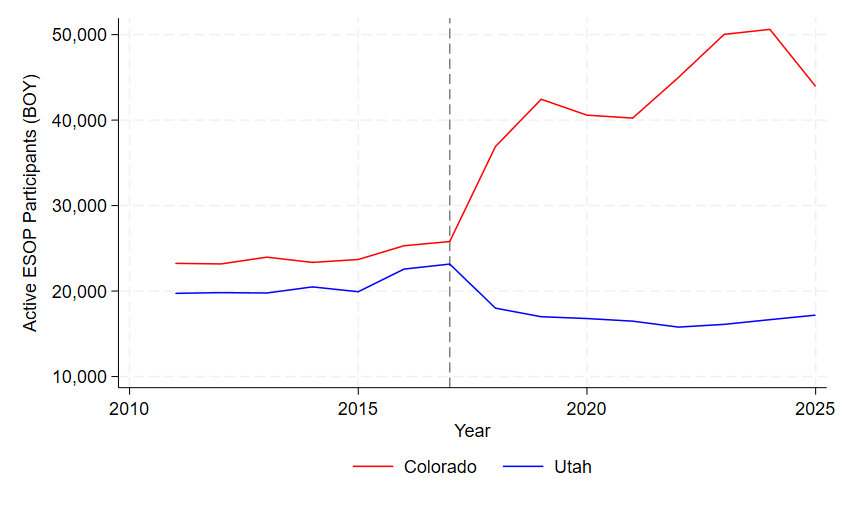
\includegraphics[width=\textwidth]{./images/data_portion/trend_comparison_tot_act_esop.png}
    \caption{Active ESOP Participants (BOY) - Colorado vs. Utah}
    \label{fig:active_participants_trend}
\end{minipage}
\hfill
\begin{minipage}{0.48\textwidth}
    \centering
    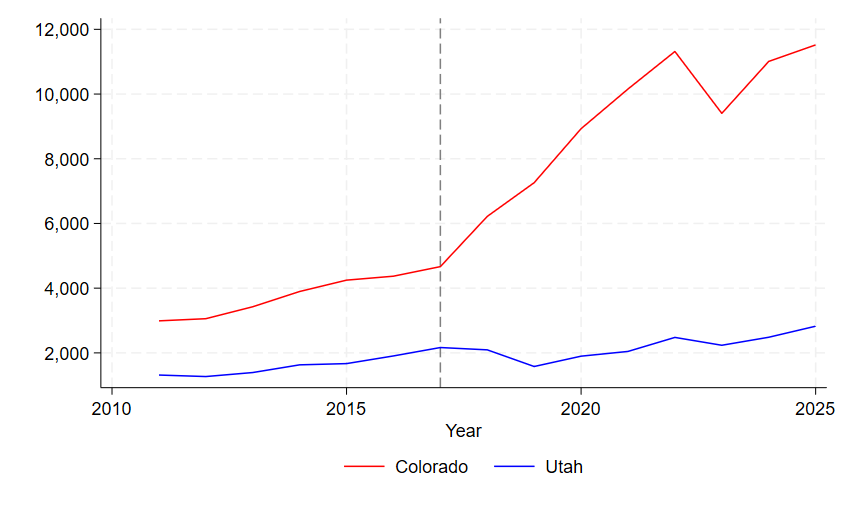
\includegraphics[width=\textwidth]{./images/data_portion/trend_comparison_esop_assets_thou.png}
    \caption{ESOP Assets EOY (Thousands USD) - Colorado vs. Utah}
    \label{fig:esop_assets_trend}
\end{minipage}
\end{figure}

Figures~\ref{fig:active_participants_trend} and~\ref{fig:esop_assets_trend} show similar trends in active ESOP participants and ESOP assets in Colorado and Utah across pre-treatment periods, with a modest increase in Colorado in 2017 compared to Utah. This motivates our further analysis of the causal relationship between the legislation passed in 2017 and ESOP participation rates in the following sections. Interestingly, Figures~\ref{fig:pension_firms_trend} and~\ref{fig:esop_firms_trend} show that trends in total firms with a pension plan and number of ESOP firms for Utah and Colorado show little to no change in the years following 2017. We discuss the potential sources for these patterns in later sections where we further explore the causal relationship.

\begin{figure}[H]
\centering
\begin{minipage}{0.48\textwidth}
    \centering
    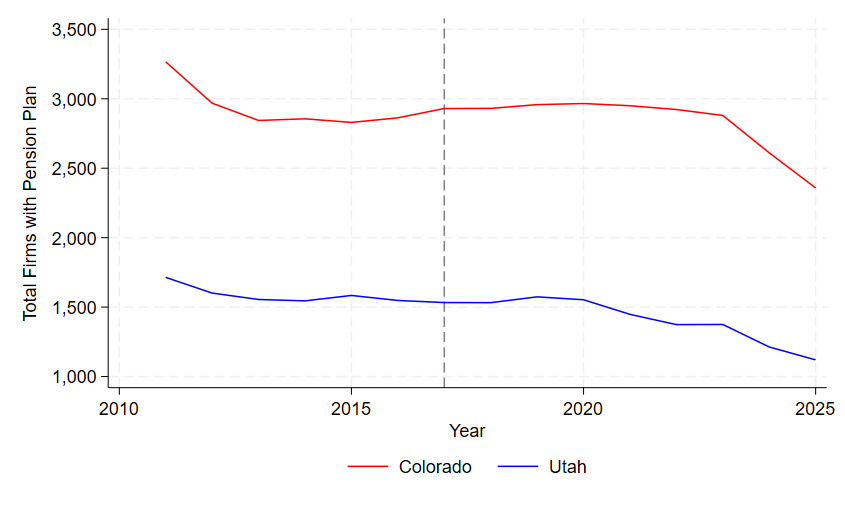
\includegraphics[width=\textwidth]{./images/data_portion/trend_comparison_total_firms.png}
    \caption{Total Firms with Pension Plan - Colorado vs. Utah}
    \label{fig:pension_firms_trend}
\end{minipage}
\hfill
\begin{minipage}{0.48\textwidth}
    \centering
    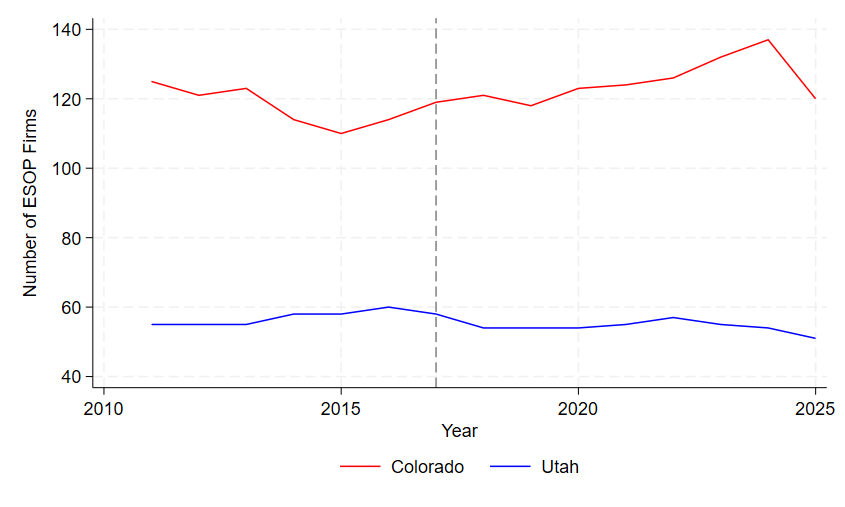
\includegraphics[width=\textwidth]{./images/data_portion/trend_comparison_num_esop_firms.png}
    \caption{Number of ESOP Firms - Colorado vs. Utah}
    \label{fig:esop_firms_trend}
\end{minipage}
\end{figure}


% III. METHODOLOGY
\section*{\centering \normalsize \textbf{III. METHODOLOGY}}

\subsection*{A. Estimation}

We employ a difference-in-differences (DiD) estimator to identify the causal effect of Colorado's HB17-1214 on ESOP participation. Our baseline specification is:

\begin{equation}
Y_{it} = \delta (\text{Colorado}_i \times \text{Post}_t) + \lambda_i + \mu_t + \epsilon_{it}
\end{equation}

where $Y_{it}$ represents one of the participation outcomes for firm $i$ in year $t$: an indicator for ESOP sponsorship, total ESOP plan participants, or total ESOP assets (measure of participation intensity). The variable $\text{Colorado}_i \times \text{Post}_t$ equals one if firm $i$ is in Colorado and year $t \geq 2017$. State fixed effects $\lambda_i$ control for time-invariant differences between Colorado and Utah, while year fixed effects $\mu_t$ absorb common shocks. The coefficient $\delta$ identifies the average treatment effect under the parallel trends assumption.

Our primary regression compares Colorado (treatment) to Utah (control), selected for its geographic proximity, similar economic structure, and absence of competing employee ownership policies during our study period.

To verify robustness, we also implement synthetic control methods (Abadie et al., 2010). We created a composite outcome constructed from the standardized forms of the outcomes of interest (Number of ESOP Firm, Total Participants, Total Active Participants, Total Assets, and ESOP participation rate)  that was averaged according to the number of outcomes being tested. This created a single combination of weights of other control states to make a synthetic Colorado. Iowa and Missouri were removed from the control states because they passed laws regarding ESOPs during the time period of interest. The weighted combination of control states minimizes the mean squared prediction error over 2012-2016. The synthetic control uses all pre-treatment outcomes in 2012, 2013, 2014, 2015, and 2016 as matching variables. 

\subsection*{B. Identification}

The validity of our DiD estimator rests on four key identifying assumptions, which we assess in turn.

\textit{Compliance.} The compliance assumption requires that treatment occurs only in the treatment group. This holds by design: HB17-1214's provisions (educational programs, loan programs, and institutional support) were enacted exclusively in Colorado and administered by the Colorado Office of Economic Development and International Trade. Utah firms had no access to these programs during 2012–2025, and Utah enacted no comparable employee ownership policies. Our analysis captures the overall effect of the policy environment on all Colorado firms, regardless of whether individual firms actively utilized the program's services. The modest observed effects may reflect low program take-up among eligible firms. Reported statistics suggest 20-25 businesses per year transitioned to employee ownership with program support, yet Colorado had approximately 118 ESOP firms pre-treatment (Table 1). This limited scale suggests either: (1) transitions involve firms too small to file Form 5500, (2) ESOP terminations offset new adoptions, or (3) the program reached only a small fraction of eligible firms.

\textit{Parallel Trends.} The parallel trends assumption requires that Colorado and Utah would have experienced the same trends in ESOP outcomes absent treatment. We test this through event study specifications:

\begin{equation}
Y_{it} = \alpha + \sum_{\substack{k=-5 \\ k \neq -1}}^{5} \beta_k \mathbbm{1}[\text{Colorado}_i \times \text{Year}_{t}^k] + \gamma_i + \lambda_t + \epsilon_{it}
\end{equation}

where $k$ indexes years relative to treatment (2017), with $k=-1$ omitted as the reference period. The coefficients $\beta_k$ for $k < 0$ test for pre-existing differential trends between Colorado and Utah.

\begin{figure}[H]
\centering
\begin{subfigure}[b]{0.48\textwidth}
    \centering
    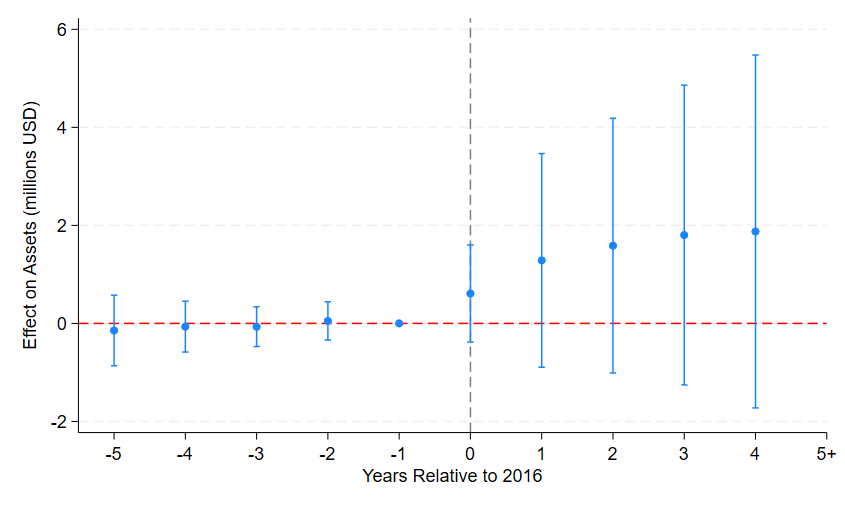
\includegraphics[width=\textwidth]{./images/data_portion/firm_event_assets_state_FE.png}
    \caption{Total ESOP Assets}
    \label{fig:event_study_1}
\end{subfigure}
\hfill
\begin{subfigure}[b]{0.48\textwidth}
    \centering
    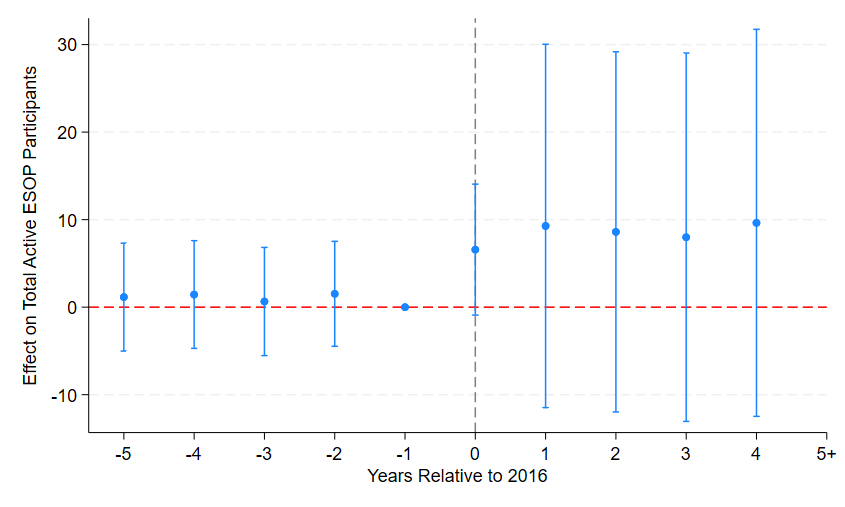
\includegraphics[width=\textwidth]{./images/data_portion/firm_event_act_partcp_state_FE.png}
    \caption{Total ESOP Participants}
    \label{fig:event_study_2}
\end{subfigure}
\caption{Event Study Results: Pre-Treatment Trends and Post-Treatment Effects}
\label{fig:event_study_both}
\end{figure}

As shown in Figure~\ref{fig:event_study_both}, pre-treatment coefficients are statistically indistinguishable from zero for both ESOP participants and assets, with coefficients clustering around zero. This provides strong evidence that Colorado and Utah exhibited parallel trends during 2012–2016. The assumption is plausible given the states' similar economic structures and shared exposure to national pension plan trends.

We cannot definitively rule out state-specific time-varying shocks after 2017 unrelated to HB17-1214. Industry-specific trends, competing state policies, or differential labor market conditions could potentially confound our estimates. For example, if Colorado's professional services sector experienced particularly strong growth after 2017 while Utah's manufacturing sector faced different trends, this could differentially affect ESOP adoption patterns independently of HB17-1214. Our state fixed effects control for time-invariant factors but cannot account for such state-specific time-varying factors. Our research identified no such contemporaneous shocks.

\textit{SUTVA (No Spillovers).} SUTVA requires that Colorado's treatment does not affect Utah outcomes. This assumption is highly plausible. First, HB17-1214's benefits require physical presence in Colorado and registration with Colorado state agencies. Small businesses rarely relocate headquarters to access such programs. Second, Form 5500 classifies firms by headquarters location. For spillovers to bias our estimates, Utah-headquartered firms would need to adopt ESOPs due to Colorado's policy while remaining headquartered in Utah. Third, ESOP transitions are complex processes involving legal restructuring and substantial costs (\$50,000–\$150,000), making them unlikely to be influenced by programs in a neighboring state.

\textit{Exclusion Restriction.} The exclusion restriction requires that HB17-1214 is the only systematic difference between Colorado and Utah after 2017 that could affect ESOP outcomes. This assumption could be violated if the policy had broader effects on Colorado's business environment or signaled state support for small businesses more generally, potentially affecting firm behavior through non-ESOP channels. However, the narrow design of HB17-1214 makes serious violations unlikely. The policy provided targeted education about employee ownership and small loans specifically for ESOP transitions, with strict eligibility criteria limiting participation to small firms (under \$5 million revenue) committed to broad-based employee ownership. The modest funding (\$200,000 annually) and technical focus suggest the policy was unlikely to generate substantial spillovers to the broader business environment or significantly shift general perceptions of Colorado as business-friendly. We reviewed Colorado legislative records and found no major retirement plan legislation, corporate tax reforms, or competing policies during 2017–2019 that would systematically affect ESOP adoption. However, we cannot definitively rule out coincidental Colorado-specific shocks, such as industry-specific trends. This untestable assumption represents the primary threat to our identification strategy.
\subsection*{C. Issues and Robustness}

Several challenges affect the validity of our estimates, though we argue these do not fundamentally undermine our central finding: Colorado's HB17-1214 had at most modest, and likely negligible, effects on ESOP participation during our study period.

\textit{Clustering and Inference:} A fundamental challenge in our design is that treatment is assigned at the state level while our outcomes are measured at the firm level. The theoretically appropriate procedure would cluster standard errors at the state level to account for correlated shocks within states over time. However, with only two states, state-level clustering is infeasible. We therefore cluster at the firm level, which accounts for serial correlation within firms but substantially understates standard errors relative to the appropriate state-level clustering. This creates a severe inference problem: our reported standard errors and p-values are likely misleading, potentially overstating the precision of our estimates. While our point estimates remain unbiased under standard DiD assumptions, we cannot reliably conduct hypothesis tests or construct confidence intervals. Importantly, this limitation works in favor of our null findings: if state-level clustering were feasible, our standard errors would be dramatically larger, making our already-insignificant results even more clearly insignificant.

\textit{Sample Size:} Our analysis compares a single treatment state (Colorado) to a single control state (Utah), providing minimal variation to identify treatment effects. This severely limits our ability to distinguish treatment effects from Colorado-specific shocks occurring after 2017. While we observe many firms within each state, the effective sample size for identifying the treatment effect is essentially two states. This constraint makes our estimates especially vulnerable to bias from any Colorado-Utah differences in post-2017 trends unrelated to HB17-1214.

\textit{Confounding Variables:} Firm participation in pension plans is highly dependent on profitability, employee turnover, competing benefit offerings, regulatory costs, and management preferences. These factors may vary systematically across states due to labor market conditions, industry composition, or unrelated state policies. If Colorado experienced differing trends in 401(k) adoption, for example, after 2017, these could mask true ESOP effects or generate spurious correlations. Our fixed effects control for time-invariant differences and common trends but cannot account for state-specific time-varying factors. Given the complex determinants of pension plan participation, small treatment effects could easily be masked by other factors influencing firms' benefit decisions.

\textit{Heterogeneous Effects.} A natural extension would be to examine whether treatment effects differ by firm size or ESOP structure type (leveraged vs. non-leveraged ESOPs). However, our dataset lacks detailed firm characteristics beyond ESOP outcomes, preventing reliable heterogeneous effect estimation. The small overall treatment effects and limited variation in our two-state design further constrain our ability to detect meaningful heterogeneity even if firm-level covariates were available. Future research with richer administrative data on firm characteristics and multi-state policy variation could productively explore whether HB17-1214 had different impacts across firm types.

While evidence supports unbiased point estimates through pre-treatment parallel trends, the reliability of our standard errors remains severely limited. With only two states, we cannot construct consistent variance estimates. Our synthetic control analysis partially addresses these concerns by constructing a counterfactual using all U.S. states as donors, which reduces dependence on Utah as the sole control. However, fundamental challenges remain.  To more definitively establish causal effects, future research should exploit multi-state designs with proper state-level clustering through: (1) a two-way fixed effects design exploiting staggered adoption of employee ownership policies across multiple states, or (2) accessing private ownership data to conduct regression discontinuity around the 30\% ESOP ownership threshold that triggers specific tax advantages. Despite these limitations, the overall pattern of small to modest effects across our firm-level and synthetic control specifications suggests minimal policy impact during our study period.

% IV. RESULTS
\section*{\centering \normalsize \textbf{IV. RESULTS}}

\subsection*{A. Main Difference-in-Differences Results}

We estimate a two-way fixed effects difference-in-differences specification comparing Colorado (treated state) and Utah (control state). Table~\ref{tab:model1} presents our baseline specification with both state and year fixed effects.

\begin{table}[H]
\centering
\caption{Difference-in-Differences Results: Year and State Fixed Effects}
\label{tab:model1}
\footnotesize

\begin{tabular}{lccccc}
\toprule
Variable & (1) ESOP Firm & (2) Total Partcps. & (3) Total Assets & (4) Active Partcps. & (5) Partcp. Rate \\
\midrule
\textbf{DID} & 0.00607 & 25.19 & 2,878,102.7* & 22.29 & 0.00613 \\
             & (0.00486) & (17.35) & (1,611,044.2) & (15.37) & (0.00426) \\
\textbf{Constant} & 0.0215*** & 18.16*** & 1,258,818.5*** & 13.99*** & 0.0175*** \\
                  & (0.00131) & (6.636) & (445,403.5) & (5.124) & (0.00113) \\
\midrule
\textbf{Observations} & 209,399 & 209,399 & 209,399 & 209,399 & 191,912 \\
\bottomrule
\end{tabular}

\vspace{0.5em}
{\footnotesize Standard errors (clustered at firm level) in parentheses. * $p<0.10$, ** $p<0.05$, *** $p<0.01$ \\
\textit{Note:} Standard errors are clustered at the firm level. Theoretically appropriate state-level clustering is infeasible with only two states.}
\end{table}

The only statistically significant result is total ESOP assets, significant at the 10\% level. We should interpret this finding cautiously because our standard errors may be understated due to clustering at the firm level rather than at the state level, where treatment was actually assigned. This potential understatement could render the result statistically insignificant under correct specification. Nevertheless, an increase of approximately \$2.88 million represents a substantial change in a firm's pension plan assets. Drawing from the summary statistics in Table 1, ESOP firms hold approximately \$32 million in assets per firm on average. Relative to this baseline, the estimated effect represents roughly a 9\% increase in total assets.
The coefficients for total participants (25.19) and active participants (22.29) are not statistically significant. However, comparing these estimates to Table 1's summary statistics, which show that Colorado ESOP firms average approximately 290 total participants, reveals that the point estimate for total participants also corresponds to about a 9\% increase. The parallel growth rates in total assets and total participants suggest internally consistent effects, even if the participation estimate lacks statistical precision. The ESOP firm indicator shows a small, insignificant increase of 0.6 percentage points (0.006 in decimal form). The participation rate results align with the firm indicator, both suggesting minimal policy impact on firm participation in ESOPs.
A key methodological note: we cluster standard errors at the firm level despite state-level treatment assignment because comparing only two states makes state-level clustering infeasible. Firm-level clustering accounts for within-firm correlation over time.

Tables~\ref{tab:model2} and~\ref{tab:model3} present robustness checks with alternative fixed effects specifications. Removing year or state fixed effects yields highly similar coefficient estimates and significance levels. The DID coefficient remains stable across specifications, indicating results are robust to the choice of fixed effects structure.

\begin{table}[H]
\centering
\caption{Difference-in-Differences Results: Year Fixed Effects Only}
\label{tab:model2}
\footnotesize
\begin{tabular}{lcccc|c}
\toprule
Variable & (1) ESOP Firm & (2) Total Partcps. & (3) Total Assets & (4) Active Partcps. & (5) Partcp. Rate \\
\midrule
\textbf{DID} & 0.00607 & 25.19 & 2,878,102.7* & 22.29 & 0.00613 \\
 & (0.00486) & (17.35) & (1,611,044.2) & (15.37) & (0.00426) \\
\textbf{Treat} & -0.00100 & -21.17 & -1,344,888.2 & -20.00 & 0.0000977 \\
 & (0.00213) & (15.07) & (1,027,215.5) & (14.25) & (0.00182) \\
\textbf{Constant} & 0.0222*** & 32.36*** & 2,160,957.6*** & 27.40*** & 0.0174*** \\
 & (0.00206) & (9.960) & (709,935.7) & (10.21) & (0.00174) \\
\midrule
\textbf{Observations} & 209,399 & 209,399 & 209,399 & 209,399 & 191,912 \\
\bottomrule
\end{tabular}

\vspace{0.5em}
{\footnotesize Standard errors (clustered at firm level) in parentheses. * $p<0.10$, ** $p<0.05$, *** $p<0.01$}
\end{table}

\begin{table}[H]
\centering
\caption{Difference-in-Differences Results: State Fixed Effects Only}
\label{tab:model3}
\footnotesize
\begin{tabular}{lcccc|c}
\toprule
Variable & (1) ESOP Firm & (2) Total Partcps. & (3) Total Assets & (4) Active Partcps. & (5) Partcp. Rate \\
\midrule
\textbf{DID} & 0.00671 & 25.59 & 2,941,710.8* & 22.47 & 0.00669 \\
 & (0.00486) & (17.29) & (1,620,237.0) & (15.18) & (0.00426) \\
\textbf{Post} & 0.0199*** & -18.67 & -778,399.0 & -18.47 & 0.0158*** \\
 & (0.00384) & (13.86) & (1,146,090.0) & (13.17) & (0.00329) \\
\textbf{Constant} & 0.0178*** & 21.52*** & 1,393,177.1*** & 17.33*** & 0.0144*** \\
 & (0.000998) & (7.304) & (485,252.2) & (6.140) & (0.000857) \\
\midrule
\textbf{Observations} & 209,402 & 209,402 & 209,402 & 209,402 & 191,915 \\
\bottomrule
\end{tabular}

\vspace{0.5em}
{\footnotesize Standard errors (clustered at firm level) in parentheses. * $p<0.10$, ** $p<0.05$, *** $p<0.01$}
\end{table}

\subsection*{B. Synthetic Control Analysis}

Using synthetic controls as a way to check robustness, we construct a counterfactual "synthetic Colorado" from weighted combinations of all other U.S. states. Figures~\ref{fig:synth_control_1}, \ref{fig:synth_control_3}, \ref{fig:synth_control_4}, and~\ref{fig:synth_control_5} display results for our four outcomes, while Table~\ref{tab:state_weights_synth} details the states and corresponding weights used to construct the synthetic Colorado. Note that Utah, our primary control state in the difference-in-differences analysis, receives zero weight in the synthetic Colorado, as its pre-treatment characteristics did not make it an optimal match for Colorado when considering all available states.

\begin{figure}[H]
\centering
\begin{minipage}{0.48\textwidth}
    \centering
    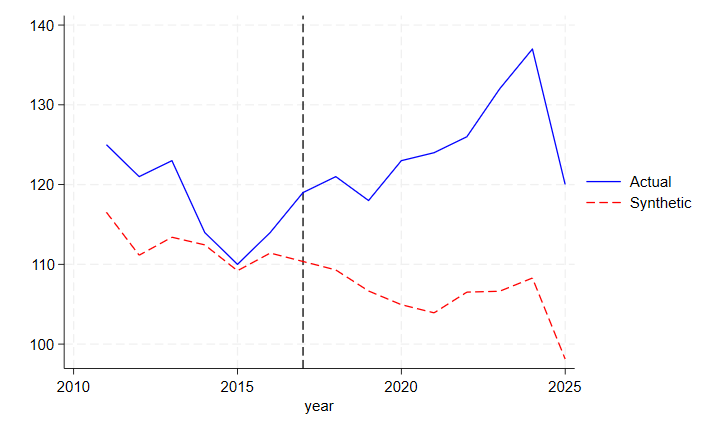
\includegraphics[width=\textwidth]{./images/esop_firms_num_synth.png}
    \caption{Synthetic Control: Number of ESOP Firms}
    \label{fig:synth_control_1}
\end{minipage}
\hfill
\begin{minipage}{0.48\textwidth}
    \centering
    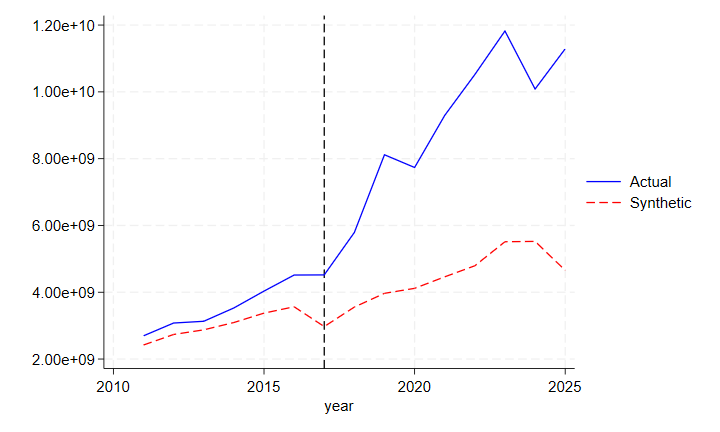
\includegraphics[width=\textwidth]{./images/esop_tot_assets_boy_amt_synth.png}
    \caption{Synthetic Control: Total ESOP Assets}
    \label{fig:synth_control_3}
\end{minipage}
\end{figure}

\begin{figure}[H]
\centering
\begin{minipage}{0.48\textwidth}
    \centering
    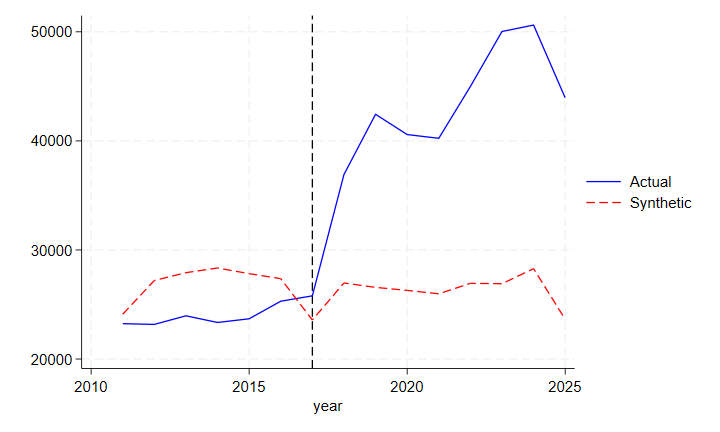
\includegraphics[width=\textwidth]{./images/esop_tot_active_partcp_cnt_synth.png}
    \caption{Synthetic Control: Active ESOP Participants}
    \label{fig:synth_control_4}
\end{minipage}
\hfill
\begin{minipage}{0.48\textwidth}
    \centering
    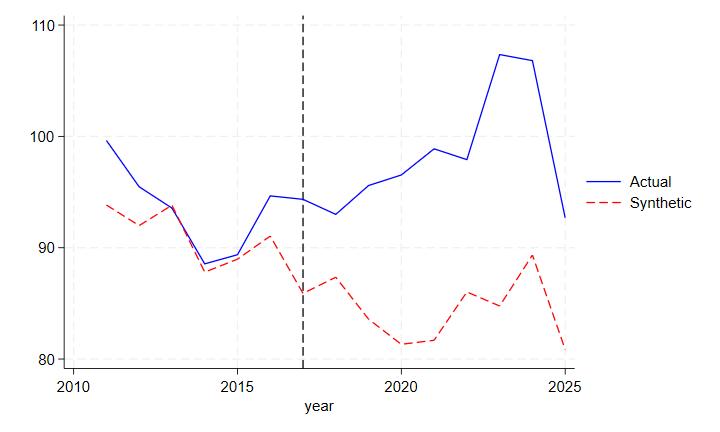
\includegraphics[width=\textwidth]{./images/esop_partcp_rate_synth.png}
    \caption{Synthetic Control: ESOP Participation Rate}
    \label{fig:synth_control_5}
\end{minipage}
\end{figure}

\begin{table}[htbp]
\centering

% ---- CAPTION ABOVE (for Table 5:) ----
\caption{\text{State Weights in the Synthetic Colorado}}
\label{tab:state_weights_synth}

% ---- TABLE CONTENT ----
\begin{tabular}{lc}
\hline
\textbf{State} & \textbf{Weight} \\
\hline
Alaska     & 0.131 \\
California & 0.361 \\
Hawaii     & 0.121 \\
Montana    & 0.387 \\
\hline
\end{tabular}

% ---- NOTE BELOW TABLE ----
\vspace{0.4em}
{\small \textit{States not included have a weight of 0.}}

\end{table}


The synthetic control estimates initially appear to suggest more substantial effects than our difference-in-differences analysis. However, closer examination of the pre-treatment fit raises concerns about the validity of these estimates. While the synthetic control methodology draws on all U.S. states to construct an optimal counterfactual for Colorado, the pre-treatment match is imperfect across several outcomes. This poor pre-treatment fit undermines the fundamental assumption that the synthetic control provides a valid counterfactual for Colorado's post-treatment trajectory. When the synthetic control fails to closely track the treated unit before intervention, post-treatment divergences may reflect pre-existing differences rather than true treatment effects.
This divergence from our difference-in-differences results, combined with the imperfect pre-treatment fit, suggests we should interpret the synthetic control estimates with considerable caution. The synthetic control approach's apparent finding of larger policy effects may be an artifact of poor pre-treatment matching rather than evidence of true treatment effects. Given these limitations and the absence of established inference procedures for synthetic controls, we view our difference-in-differences estimates as more reliable, despite their own limitations. The contrasting findings between methodologies underscore the need for future multi-state studies with greater statistical power and more robust identification strategies.
% V. CONCLUSION
% V. CONCLUSION
\section*{\centering \normalsize \textbf{V. CONCLUSION}}

\vspace{12pt}

We find limited evidence that Colorado's HB17-1214 significantly increased ESOP participation during 2012-2019. Our two-way fixed effects estimates show small and mostly insignificant effects across all outcomes, with only total ESOP assets marginally significant at the $10\%$ level (\$2.9 million increase). While synthetic controls initially suggested somewhat larger effects, poor pre-treatment fit across outcomes undermines confidence in these estimates, making the apparent post-treatment divergences difficult to interpret as causal effects. We therefore place greater weight on our difference-in-differences estimates.
Our analysis faces severe identification constraints. Most critically, with only two states, we cannot implement appropriate state-level clustering of standard errors, substantially understating true uncertainty. We cannot rule out Colorado-specific trends after 2017 that could confound our estimates. Fundamentally, comparing two states provides minimal statistical power to detect modest policy effects. Several factors may explain our null findings: the policy focused on education rather than direct financial incentives, targeted only small businesses under \$5 million revenue, and we likely miss smaller ESOPs below Form 5500 reporting thresholds.

Future research should exploit staggered adoption of employee ownership policies across multiple states to enable proper state-level inference and greater statistical power. Additionally, accessing administrative data on ESOP formations and linked employer-employee records would allow comprehensive analysis of both firm-level adoption and employee-level outcomes. Our analysis demonstrates both the promise of Form 5500 data for studying employee ownership and the fundamental challenges of evaluating state policies with limited cross-sectional variation.

% Prof. Wilson: Would be helpful to see table with weights. Where is Utah?


% References
\section*{\centering \normalsize \textbf{VI. REFERENCES}}
% Prevent the bibliography environment from printing its own heading (avoid double 'References')
\renewcommand{\bibsection}{}
\bibliographystyle{apalike}
\nocite{*}
\bibliography{references}

\end{document}